\section{Problem Description}
In order to realize a directional low-mid emission with the chosen speaker configuration, signal parameters have to be chosen in a specific manner. The directional characteristics of the speaker array depend on the amplitude and phase of the signal that is transduced via the individual speakers. The resulting directional characteristics of a given set of signal-parameters can be described by the use of a analytical model, that has been supplemented with knowledge from measuring the polar response of the speakers.\\
Assuming, that the model describing the directional characteristics of the array is sufficiently accurate, it is possible to form an optimization problem. Any set of \gls{sp} parameters can be evaluated by plugging it into the supplemented analytical model, which will be used to form an objective function. Solutions, that resemble the desired directional characteristic are considered optimal.\\
The supplemented analytical model describes intricate physical behaviour and is related to the desired behaviour of the speaker array.  This makes it favourable to approach the given problem with combinatorial optimization. Specifically, it has been chosen to handle the problem with a \gls{ga}, where the supplemented analytical model used to evaluate the \textit{fitness}.


\section{\gls{ga}: Fundamentals}
In \citep[p. 7]{goldberg89} theAdding \(S\) to the distance between the front plane of the cabinet and the rotational axis, a rough estimate of the position of the acoustic center in relation to the front plane of the cabinet \(C\,\approx\,\)\SI{0.17}{\meter} can be made. As there were still some mechanical weaknesses involved and the temperature during the measurement was unknown, this estimate has to be confirmed in a final measurement campaign, where the speaker is set back according to the findings of \autoref{tab:shift_meas2}.\\
 author designates four main properties in order to elucidate genetic algorithms. 
\begin{itemize}
\item \gls{ga}s rely on coded parameter sets, not the natural parameters themselves.
\item \gls{ga}s work with a \textit{population} of solutions, not a single one.
\item \gls{ga}s only require an objective function to evaluate the fitness of the solutions, not its derivative or other auxilary information.
\item \gls{ga}s utilize probabilistic transition rules for generating new solutions, as opposed to determinstic transistions.
\end{itemize}
These points outline the fundamental idea of a \gls{ga}s. A pool of solutions to a given problem evolves over a number of generations via probabilistic transition rules (\textit{crossover}, \textit{mutation}).
These transition rules rely on evaluating the fitness of the solutions with the objective function in order to adjust the probabilities so that desirable properties are likely to subsist.
\citep{genetic_survey}

\section{Optimization Results}\label{sec:opt_result}
\begin{figure}[H]
	\centering
	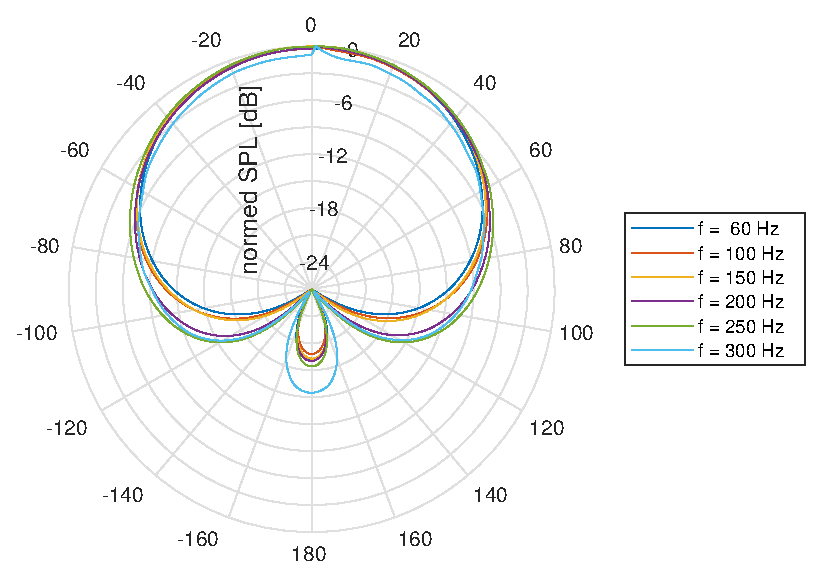
\includegraphics[width=0.7\textwidth]{expected_polar_pcor.eps}
	\caption{Expected directional characteristics, optimization with pressure corrected cost function, correction table based on Appendix \ref{ax:directional_2}, generation count: $n_{start}=60$, $n_{rest}=30$, population size $t=1250$}
		\label{fig:expected_pcor}
\end{figure}